% latex $fileNameWithoutExt; dvisvgm $fileNameWithoutExt --bbox=papersize --font-form=ttf --precision=3 --optimize=collapse-groups,group-attributes,simplify-text,simplify-transform
\documentclass[tikz, border=2mm]{standalone}
\usetikzlibrary{matrix}
\usetikzlibrary{positioning}
\begin{document}
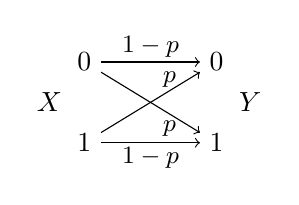
\begin{tikzpicture}
  \matrix (m) [matrix of nodes, column sep=36px, row sep=16px]
  {
    0 & 0 \\
    1 & 1 \\
  };
  \node[left of=m, left=0px] {$X$};
  \node[right of=m, right=0px] {$Y$};
  \path[->, font=\small]
  (m-1-1) edge node [above=-2px] {$1-p$} (m-1-2)
  (m-1-1) edge node [below right=3px and 1px] {$p$} (m-2-2)
  (m-2-1) edge node [above right=2px and 1px] {$p$} (m-1-2)
  (m-2-1) edge node [below=-2px] {$1-p$} (m-2-2);
\end{tikzpicture}
\end{document}
